\documentclass[12pt]{article}
\usepackage[a4paper,margin=0.75in]{geometry}
\usepackage[utf8]{inputenc}
\usepackage[OT1]{fontenc}
\usepackage[table,usenames,dvipsnames]{xcolor}
\usepackage{array}
\usepackage{varwidth}
\usepackage{tabularx}
\usepackage{amsmath}
\usepackage{hyperref}
\usepackage{enumitem}
\usepackage{graphicx}
\usepackage{tcolorbox}
\renewcommand*\familydefault{\sfdefault}

\newtcolorbox{mybox}[3][]
{
  colframe = #2!25,
  colback  = #2!10,
  coltitle = #2!20!black,  
  title    = {#3},
  #1,
}

\hypersetup{
    colorlinks=true,
    linkcolor=blue,
    filecolor=magenta,      
    urlcolor=cyan,
    pdftitle={Overleaf Example},
    pdfpagemode=FullScreen,
}

\title{\textbf{COL774 Assignment 2}}
\author{Aman Hassan \\ \texttt{2021CS50607}}
\date{October 2023}

\begin{document}

\maketitle

\section{Naive Bayes}

\begin{enumerate}[label=(\alph*)]
  
    \item Here we implemented Naive Naive Bayes that uses the \textbf{Multinoulli distribution/Multinomial distribution}
    \begin{enumerate}[label=\roman*.]
        \item 
            \begin{itemize}
                \item Time taken for parameter finding:4.943481206893921
                \item Time taken for prediction:25.203924417495728
                \item Accuracy in Training set using naive bayes = 0.8504648214663004
                \item Time taken for parameter finding:5.051173686981201
                \item Time taken for prediction:2.271172523498535
                \item Accuracy in Validation set using naive bayes = 0.6705132098390525
            \end{itemize}
        \item The following word clouds were obtained for each class
    \end{enumerate}
    \begin{center}
        \begin{tabular}{c c c}
            
\includegraphics[width=0.3\textwidth]{Images/Q1/a/ptext.png} & 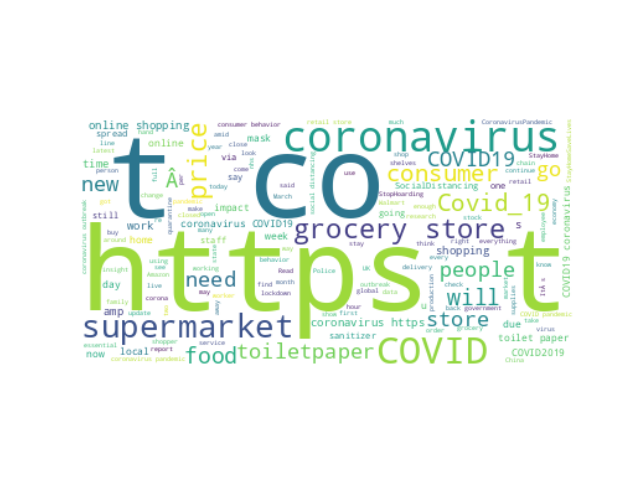
\includegraphics[width=0.3\textwidth]{Images/Q1/a/neutext.png} &
            \includegraphics[width=0.3\textwidth]{Images/Q1/a/ntext.png} \\
            Positive  & Neutral & Negative
        \end{tabular}
    \end{center}
    
    \item With Random Guessing, we should expect a 33\% accuracy on average which is also what we observe (A particular run gave 33.73823261463711\% accuracy). By predicting positive always we see that prediction accuracy is 43.85059216519891 because of the higher number of positive tweets over others.

    The Part a) of Naive Bayes gives us 98.73987398739874\% gain over Random Guessing (i.e. Naive Bayes is almost twice better than random) and gives 52.908587257617704\% gain over simply predicting positive.

    \item \begin{itemize}
        \item The confusion matrices for training set are as follows:
        \begin{center}
            \begin{tabular}{c c}
                NaiveBayes & Random \\
                \begin{tabular}{r|c|c|c}
                    & AP & ANu & AN \\
                    \hline
                    PP & 15711 & 2158 & 1078\\
                    \hline
                    PNu & 177 & 3574 & 171 \\
                    \hline
                    PN & 714 & 1364 & 12917 \\
                    \hline
                \end{tabular} & 
                \begin{tabular}{r|c|c|c}
                    & AP & ANu & AN \\
                    \hline
                    PP & 5385 & 2415 & 4747\\
                    \hline
                    PNu & 5595 & 2359 & 4703 \\
                    \hline
                    PN & 5622 & 2322 & 4716 \\
                    \hline
                \end{tabular}
            \end{tabular}
            \end{center}
            \begin{center}
            \begin{tabular}{c}
                All Positive \\
                \begin{tabular}{r|c|c|c}
                    & AP & ANu & AN \\
                    \hline
                    PP & 16602 & 7096 & 14166\\
                    \hline
                    PNu & 0 & 0 & 0 \\
                    \hline
                    PN & 0 & 0 & 0 \\
                    \hline
                \end{tabular}
            \end{tabular}
            \end{center}
        \item The confusion matrices for validation set are as follows:
        \begin{center}
            \begin{tabular}{c c}
                NaiveBayes & Random \\
                \begin{tabular}{r|c|c|c}
                    & AP & ANu & AN \\
                    \hline
                    PP & 1121 & 271 & 272\\
                    \hline
                    PNu & 77 & 174 & 55 \\
                    \hline
                    PN & 246 & 174 & 905 \\
                    \hline
                \end{tabular} & 
                \begin{tabular}{r|c|c|c}
                    & AP & ANu & AN \\
                    \hline
                    PP & 479 & 206 & 415\\
                    \hline
                    PNu & 468 & 186 & 225 \\
                    \hline
                    PN & 497 & 409 & 408 \\
                    \hline
                \end{tabular}
            \end{tabular}
            \end{center}
            \begin{center}
            \begin{tabular}{c}
                All Positive \\
                \begin{tabular}{r|c|c|c}
                    & AP & ANu & AN \\
                    \hline
                    PP & 1444 & 617 & 1232\\
                    \hline
                    PNu & 0 & 0 & 0 \\
                    \hline
                    PN & 0 & 0 & 0 \\
                    \hline
                \end{tabular}
            \end{tabular}
            \end{center}
    \end{itemize}


    We can see that for Naive Bayes classifier, the number of correctly predicted samples (i.e. the trace of confusion matrix) is higher than the others which indicates that Naive Bayes classifier has a higher prediction accuracy than random or positive guessing

    Note that on adding the values in the entire matrix we get back total number of training examples and adding up a particular column value gives us the total number of actual training examples in that class.

    \item The following transformations were done in this part:
    \begin{itemize}
        \item Remove \#'s and @'s (and their corresponding tags)
        \item Remove special chars like !, . , * etc
        \item Stopword removal
        \item Lemmatize
    \end{itemize}

    \begin{center}
        \begin{center}
        \begin{tabular}{c c c}
            
\includegraphics[width=0.3\textwidth]{Images/Q1/d/ptext.png} & 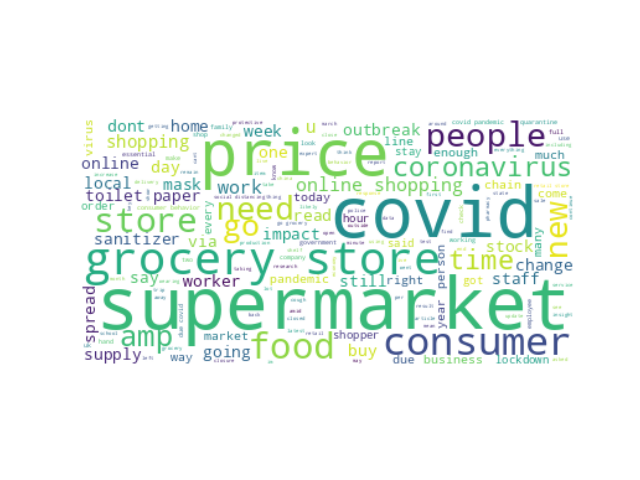
\includegraphics[width=0.3\textwidth]{Images/Q1/d/nutext.png} &
            \includegraphics[width=0.3\textwidth]{Images/Q1/d/ntext.png} \\
            Positive  & Neutral & Negative
        \end{tabular}
    \end{center}
    \end{center}

    The output accuracy produced was:
    \begin{itemize}
        \item Naive Bayes prediction accuracy with basic data cleaning = 0.6680838141512299
        \item Naive Bayes prediction accuracy with better data cleaning (stemming) = 0.7060431217734588
        \item Naive Bayes prediction accuracy with better data cleaning (lemmatizing) = 0.7127239599149712
    \end{itemize}

    Some observations to note:
    \begin{itemize}
        \item The word clouds show the frequency of the various lemma of words rather than the frequency of the words themselves.
        \item Accuracy increases since the data has lesser noise compared to earlier which allows for better predictions
        \item Lemmatizing has better accuracy over stemming
    \end{itemize}
    


\item Bigrams has not been implemented:
% Using Bigrams (in addition to removing stopwords and stemming) gives us an accuracy of \textbf{84.4 \%}, with 8209/10000 positive reviews and 4447/5000 negative reviews correctly classified.

%     For the additional feature, we use Trigrams. Using trigrams, in addition to bigrams and removing stopwords + stemming gives us an accuracy of \textbf{85.2 \%}, with 8352/10000 positive reviews and 4423/5000 negative reviews correctly classified.

%     The additional sets of features do help us improve our accuracy (explain why)

\item Using Domain adaptation the following results were obtained:

\begin{enumerate}[label=\roman*.]
    \item Using Source Data:
    \begin{itemize}
        \item The prediction accuracy when using split 1 with source domain is 47.97879390324719
        \item The prediction accuracy when using split 2 with source domain is 48.31013916500994
        \item The prediction accuracy when using split 5 with source domain is 48.70775347912525
        \item The prediction accuracy when using split 10 with source domain is 50.132538104705105
        \item The prediction accuracy when using split 25 with source domain is 50.56328694499669
        \item The prediction accuracy when using split 50 with source domain is 51.789264413518886
        \item The prediction accuracy when using split 100 with source domain is 54.208084824387015
    \end{itemize}
    \item Without using Source Data:
    \begin{itemize}
        \item The prediction accuracy when using split 1 is 34.327369118621604
        \item The prediction accuracy when using split 2 is 35.387673956262425
        \item The prediction accuracy when using split 5 is 39.72829688535454
        \item The prediction accuracy when using split 10 is 44.26772697150431
        \item The prediction accuracy when using split 25 is 46.02385685884692
        \item The prediction accuracy when using split 50 is 49.07223326706428
        \item The prediction accuracy when using split 100 is 52.51822398939695
    \end{itemize}
    \item The obtained graph is as follows:
     \begin{center}\raisebox{-.9\height}{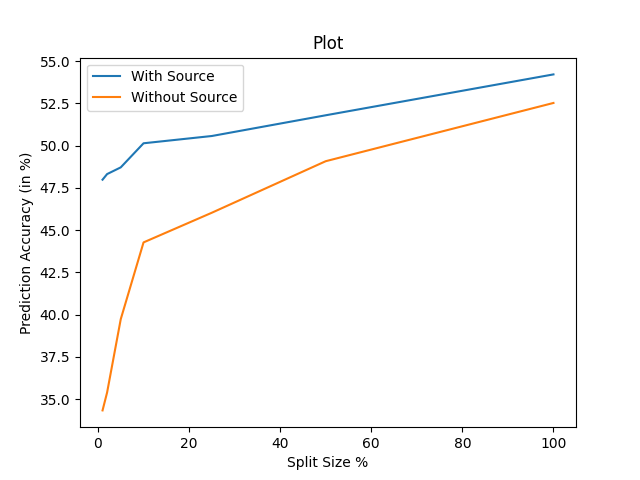
\includegraphics[width=0.7\textwidth]{Images/Q1/f/Source_vs_NoSource.png}}\end{center}
    \newpage
    \item Observations to note:
    \begin{itemize}
        \item We see that the prediction accuracy using source data is higher than the prediction accuracy without source data
        \item Initially the model without source data performs considerably worse compared to the one using source data. This can possibly be attributed to the fact that the intial splits have very less data because of which intial model without souce data cannot predict accurately.
        \item As the split size increases the model without source data approaches the accuracy of the one with source data. This can possibly be attributed to the fact that the model without source data is more generalised and can hence predict better compared to the source data model which has been trained against Corona specific tweets.
        \item Both models reach just above 50\% accuracy.This can possibly be attributed the fact that there are not info datapoints to train the model accurately (ie small size of general tweet training set compared to Corona training set). Possibly also due to the fact that many tweets in the general tweet training set are repeated and just subsets of other tweets.

    \end{itemize}
\end{enumerate}


\end{enumerate}

\clearpage

\section{Binary SVM}

\begin{enumerate}[label=(\alph*)]
    \item \begin{enumerate}[label=\roman*.]
        \item With a threshold of $\alpha_i > 10^{-6}$ for the support vectors. We obtain the following results for a linear kernel
        \begin{itemize}
            \item No of support vectors: 673
            \item \% of support vectors wrt training examples: 14.138655462184873\%
        \end{itemize}
        \item The test accuracy we obtain is 94.0\%
        \item The top 6 support vectors are:

        \begin{center}
        \begin{tabular}{c c c}
            
\includegraphics[width=0.2\textwidth]{Images/Q2_binary/linear_sv_1.png} &
            
\includegraphics[width=0.2\textwidth]{Images/Q2_binary/linear_sv_2.png} &
            
\includegraphics[width=0.2\textwidth]{Images/Q2_binary/linear_sv_3.png} \\
        \end{tabular}
        \begin{tabular}{c c c}
            
\includegraphics[width=0.2\textwidth]{Images/Q2_binary/linear_sv_4.png} &
            
\includegraphics[width=0.2\textwidth]{Images/Q2_binary/linear_sv_5.png} &
            
\includegraphics[width=0.2\textwidth]{Images/Q2_binary/linear_sv_6.png} \\
        \end{tabular}
        \end{center}

        The weight image obtained is:

        \begin{center}
            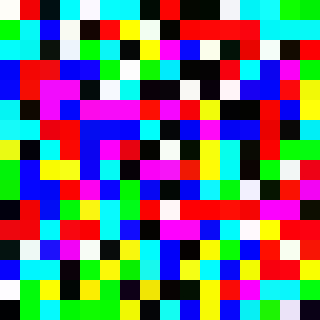
\includegraphics[width=0.2\textwidth]{Images/Q2_binary/linear_w.png} 
        \end{center}
    \end{enumerate}

    \item \begin{enumerate}[label=\roman*.]
        \item With a threshold of $\alpha_i > 10^{-6}$ for the support vectors. We obtain the following results for a Gaussian Kernel
        \begin{itemize}
            \item No of support vectors: 1067
            \item \% of support vectors wrt training examples: 22.415966386554622\%
            \item Number of support vectors that match in both linear and gaussian: 571
        \end{itemize}
        \item The test accuracy we obtain is 94.25\%
        \item The top 6 support vectors are:

        \begin{center}
        \begin{tabular}{c c c}
            
\includegraphics[width=0.2\textwidth]{Images/Q2_binary/gaussian_sv_1.png} &
            
\includegraphics[width=0.2\textwidth]{Images/Q2_binary/gaussian_sv_2.png} &
            
\includegraphics[width=0.2\textwidth]{Images/Q2_binary/gaussian_sv_3.png} \\
        \end{tabular}
        \begin{tabular}{c c c}
            
\includegraphics[width=0.2\textwidth]{Images/Q2_binary/gaussian_sv_4.png} &
            
\includegraphics[width=0.2\textwidth]{Images/Q2_binary/gaussian_sv_5.png} &
            
\includegraphics[width=0.2\textwidth]{Images/Q2_binary/gaussian_sv_6.png} \\
        \end{tabular}
        \end{center}
    \item We see that the validation accuracy obtained in Gaussian kernel is slightly higher than that of linear kernel (0.25\% higher)
    \end{enumerate}

    \item \begin{enumerate}[label=\roman*.]
        \item Number of Support Vectors obtained is as follows
        \begin{itemize}
            \item Linear Kernel: sklearn\_svm has 669 SV's over CVXOPT's 673 SV's
            \item Gaussian Kernel: sklearn\_svm has 1056 SV's over CVXOPT's 1067 SV's
        \end{itemize}
        \begin{center}
            \begin{tabular}{c c}
                & CVXOPT \\
                Scikit & 
            \begin{tabular}{c|c|c|}
                    & lin  & rbf  \\   
                \hline
                lin & 669 & 569 \\
                \hline
                rbf & 566 & 1056 \\
                \hline
            \end{tabular}
            \end{tabular}
        \end{center}

    \item Comparison of weight and bias in linear kernel:
    \begin{itemize}
        \item CVXOPT: b = -4.0888424817486575
        \item sklearn\_svm: b = -4.0881856782113015
        \item norm(w\_cv - w\_skl) = 0.015257845622513772
    \end{itemize}
    \item Validation set accuracy is as follows:
    \begin{itemize}
        \item Linear Kernel: sklearn\_svm obtains 94.75\% accuracy over CVXOPT's 94\% accuracy
        \item Gaussian Kernel: sklearn\_svm obtains 93.75\% accuracy over CVXOPT's 94.25\% accuracy
    \end{itemize}

        \item The training times are given below:
            \begin{center}
                \begin{tabular}{|l|c|}
                    \hline
                    Scikit RBF & 1.649s (+ 23.210s for data retrieval) \\
                    Scikit linear & 1.944s (+ 22.590s for data retrieval)\\
                    CVXOPT RBF & 154.257s (+ 23.080s for data retrieval)\\
                    CVXOPT linear & 81.493s (+ 24.363s for data retrieval)\\
                    \hline
                \end{tabular}
            \end{center}
    \end{enumerate}

\end{enumerate}

\section{Multiclass SVM}

\begin{enumerate}[label=(\alph*)]
    \item Using the previously created CVXOPT Solver we obtain 55.414\% accuracy in Multi-class classification
    \item Using the scikit SVM library we obtain 56.083\% accuracy on the same test set. We also see that in comparison to CVXOPT, the scikit SVM library is much faster. The exact time taken to train the model is as follows 2028.495s (\~ 33 mins) for CVXOPT implementation in comparison to 53.316s (\~ 1 min) for scikit library. Note the accuracy rate is almost similar (differing only by \~0.53\%)

    \item The confusion matrices for both implementations is as follows:
    \begin{center}
        \begin{tabular}{c c}
            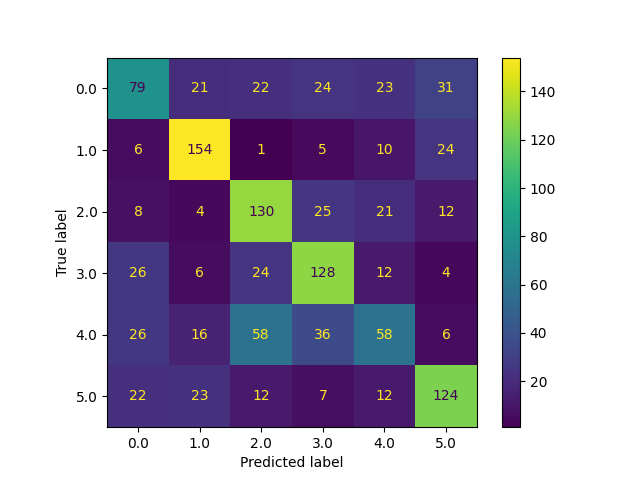
\includegraphics[width=0.44\textwidth]{Images/Q2_multi/confusion_sklearn.png} & 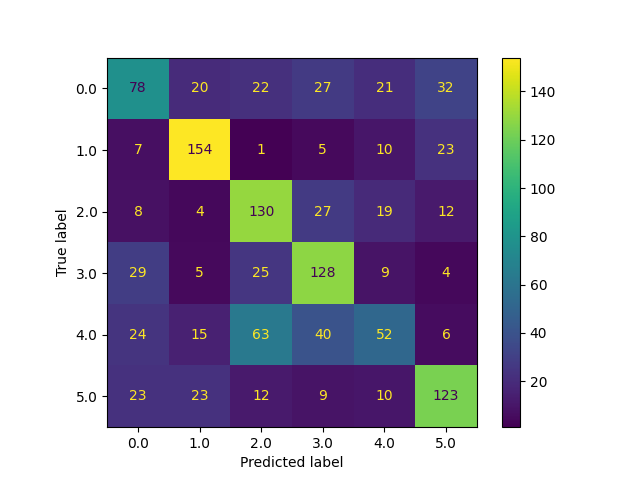
\includegraphics[width=0.44\textwidth]{Images/Q2_multi/confusion_cvxopt.png} \\
            Scikit & CVXOPT 
        \end{tabular}
    \end{center}

   We observe that classes 0 and 4 are the most misclassified classes with class 4 getting misclassified as class 2 or class 3 and class 0 getting misclassified as class 5. Below, we plot first 12 examples which are misclassified by Scikit and CVXOPT (both turn out to be the same), with their {\color{red} predicted} and {\color{green} original} labels respectively

    \begin{center}
        \setlength\tabcolsep{1pt}
        \begin{tabular}{c c c c c c c c c c c c c}
            &
            
\includegraphics[width=0.065\textwidth]{Images/Q2_multi/misclassified/sklearn1_5_0.png} &
            
\includegraphics[width=0.065\textwidth]{Images/Q2_multi/misclassified/sklearn2_5_0.png} &
            
\includegraphics[width=0.065\textwidth]{Images/Q2_multi/misclassified/sklearn3_4_0.png} &
            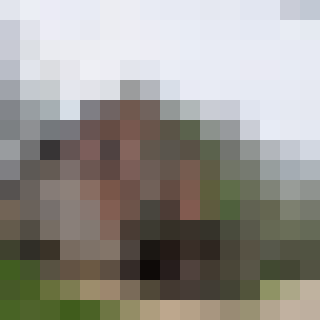
\includegraphics[width=0.065\textwidth]{Images/Q2_multi/misclassified/sklearn4_3_0.png} &
            
\includegraphics[width=0.065\textwidth]{Images/Q2_multi/misclassified/sklearn5_5_0.png} &
            
\includegraphics[width=0.065\textwidth]{{Images/Q2_multi/misclassified/sklearn6_2_0.png}} &
            
\includegraphics[width=0.065\textwidth]{Images/Q2_multi/misclassified/sklearn7_3_0.png} &
            
\includegraphics[width=0.065\textwidth]{Images/Q2_multi/misclassified/sklearn8_4_0.png} &
            
\includegraphics[width=0.065\textwidth]{Images/Q2_multi/misclassified/sklearn9_3_0.png} &
            
\includegraphics[width=0.065\textwidth]{Images/Q2_multi/misclassified/sklearn10_3_0.png} &
            
\includegraphics[width=0.065\textwidth]{Images/Q2_multi/misclassified/sklearn11_3_0.png} &
            
\includegraphics[width=0.065\textwidth]{Images/Q2_multi/misclassified/sklearn12_5_0.png} \\
            SK: &
            {\color{red} 0} {\color{green} 5} &
            {\color{red} 0} {\color{green} 5} &
            {\color{red} 0} {\color{green} 4} &
            {\color{red} 0} {\color{green} 3} &
            {\color{red} 0} {\color{green} 5} &
            {\color{red} 0} {\color{green} 2} &
            {\color{red} 0} {\color{green} 3} &
            {\color{red} 0} {\color{green} 4} &
            {\color{red} 0} {\color{green} 3} &
            {\color{red} 0} {\color{green} 3} &
            {\color{red} 0} {\color{green} 3} &
            {\color{red} 0} {\color{green} 5} \\
            &
            
\includegraphics[width=0.065\textwidth]{Images/Q2_multi/misclassified/cvxopt1_5_0.png} &
            
\includegraphics[width=0.065\textwidth]{Images/Q2_multi/misclassified/cvxopt2_5_0.png} &
            
\includegraphics[width=0.065\textwidth]{Images/Q2_multi/misclassified/cvxopt3_4_0.png} &
            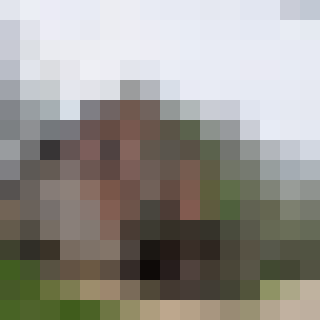
\includegraphics[width=0.065\textwidth]{Images/Q2_multi/misclassified/cvxopt4_3_0.png} &
            
\includegraphics[width=0.065\textwidth]{Images/Q2_multi/misclassified/cvxopt5_5_0.png} &
            
\includegraphics[width=0.065\textwidth]{{Images/Q2_multi/misclassified/cvxopt6_2_0.png}} &
            
\includegraphics[width=0.065\textwidth]{Images/Q2_multi/misclassified/cvxopt7_3_0.png} &
            
\includegraphics[width=0.065\textwidth]{Images/Q2_multi/misclassified/cvxopt8_4_0.png} &
            
\includegraphics[width=0.065\textwidth]{Images/Q2_multi/misclassified/cvxopt9_3_0.png} &
            
\includegraphics[width=0.065\textwidth]{Images/Q2_multi/misclassified/cvxopt10_3_0.png} &
            
\includegraphics[width=0.065\textwidth]{Images/Q2_multi/misclassified/cvxopt11_3_0.png} &
            
\includegraphics[width=0.065\textwidth]{Images/Q2_multi/misclassified/cvxopt12_5_0.png} \\
            CVXOPT: &
            {\color{red} 0} {\color{green} 5} &
            {\color{red} 0} {\color{green} 5} &
            {\color{red} 0} {\color{green} 4} &
            {\color{red} 0} {\color{green} 3} &
            {\color{red} 0} {\color{green} 5} &
            {\color{red} 0} {\color{green} 2} &
            {\color{red} 0} {\color{green} 3} &
            {\color{red} 0} {\color{green} 4} &
            {\color{red} 0} {\color{green} 3} &
            {\color{red} 0} {\color{green} 3} &
            {\color{red} 0} {\color{green} 3} &
            {\color{red} 0} {\color{green} 5} \\
        \end{tabular}
    \end{center}

    The classes of the Intel Image dataset are Building(0), Forest(1), Glacier(2), Mountain(3), Ocean(4) and Road(5). The model(s) misclassify several examples in the Building and Road categories amongst each other, which makes sense because most of the images with roads are surrounded by buildings. Similarly, Ocean seems to be misclassified into Glacier's as well, which also makes sense since the backgrounds are similar.

    \item The obtained accuracies are as follows:
    \begin{itemize}
        \item K-fold cross verification: [15.342\%, 15.671\%, 54.263\%,56.132\%,58.679\%]
        \item Validation accuracy [41.240\%, 41.368\%, 53.482\%,56.726\%,58.629\%]
    \end{itemize}
    \item The obtained graph is given in the following page. The value of determines the number of misclassifications, a higher value of C would provide less misclassification but with the downside that it would tend to overfit. Smaller values of C underfit the model and causes a poor decision boundary which is exactly what we obtained as per the graph.
    We also see that both K-fold and validation classify better the higher the value of C.

        \begin{center}
            \includegraphics[width=0.7\textwidth]{Images/Q2_multi/Accuracy_vs_C.png}
        \end{center}

\end{enumerate}

\end{document}